
\section{Grain charging and gas--grain coupling around OB stars}
\label{sec:cloudy-models-dust}

We calculate models of the physical properties of dust grains using
the plasma physics code Cloudy \citep{Ferland:2013a, Ferland:2017a},
which self-consistently solves the multi-frequency radiative transfer
together with thermal, ionization, and excitation balance of all
plasma constituents.  Cloudy incorporates grain charging as described
in \citet{Baldwin:1991a} and \citet{van-Hoof:2004a} with photoelectric
emission theory from \citet{Weingartner:2001b, Weingartner:2006a}.  We
use the default ``ISM'' dust mixture included in Cloudy, which
comprises ten size bins each for spherical silicate and graphite
grains in the range \num{0.005} to \SI{0.25}{\um}, and which is
designed to reproduce the average Galactic extinction curve
\citep{Weingartner:2001a, Abel:2008a}.  The optical properties of each
grain species are calculated using Mie theory \citep{Bohren:1983a},
assuming solid spheres.  The resultant wavelength-dependent extinction
properties of the mixture are summarised in
Figure~\ref{fig:cloudy-ism-dust-opacity}.

\begin{figure}
  \centering
  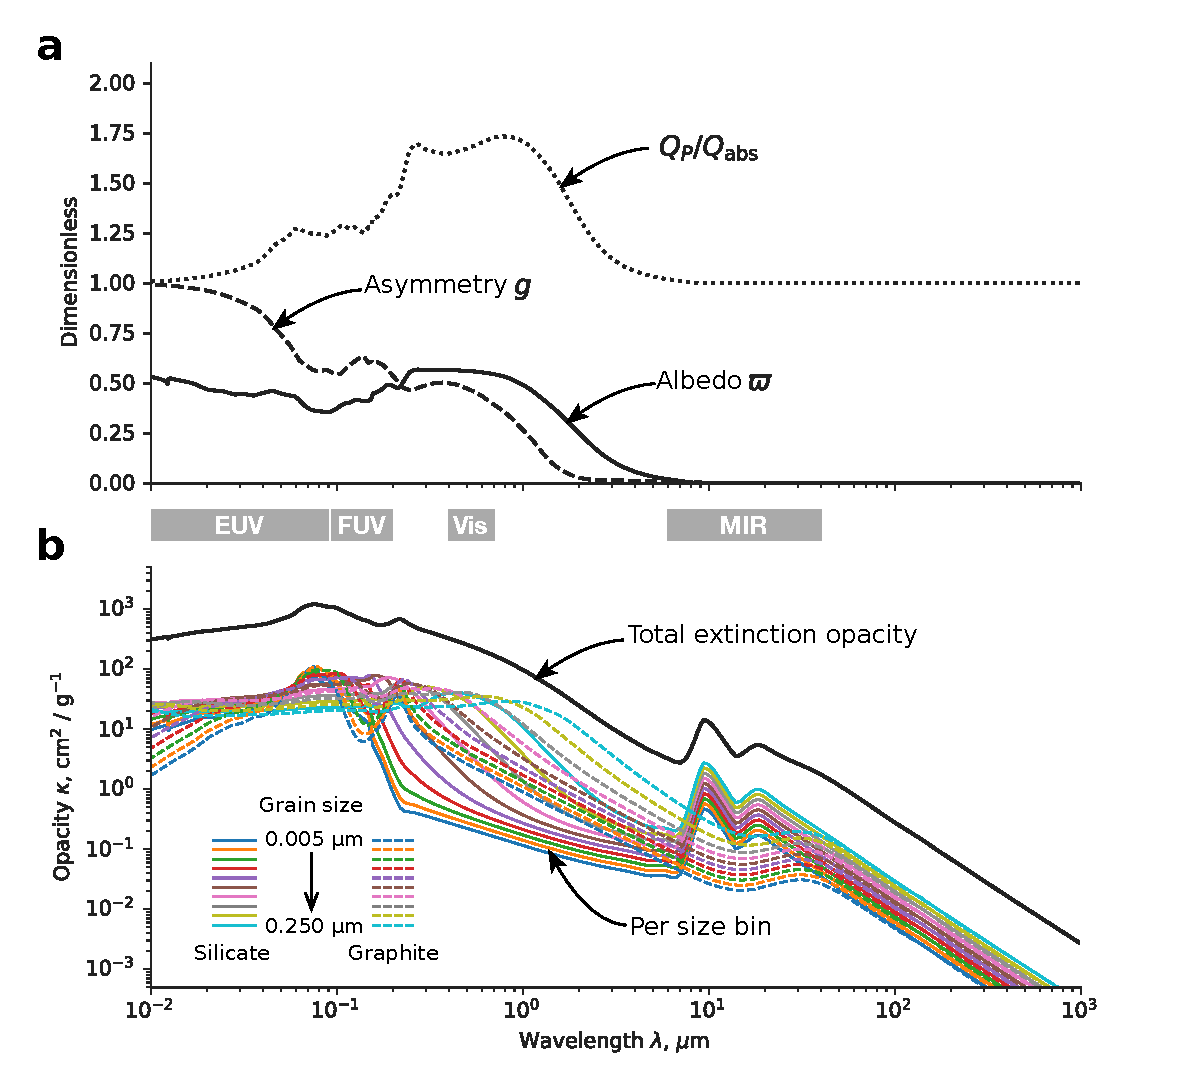
\includegraphics[width=\linewidth]{figs/cloudy-ism-dust-opacity}
  \caption{Extinction properties of Cloudy's standard ``ISM'' dust
    mixture. %
    (a)~Wavelength dependence of mean values over the entire mixture
    of three dimensionless quantities related to scattering: albedo,
    \(\varpi\) (solid line); scattering asymmetry,
    \(g = \langle \cos\theta \rangle\) (dashed line); ratio of radiation pressure
    efficiency to absorption efficiency, \(Q_P / Q_{\text{abs}}\)
    (dotted line).
    %
    (b)~Wavelength dependence of mass opacity (cross section per unit
    mass of gas) for the whole mixture (heavy black line) and broken
    down by size bin and grain composition (colored lines, see key). }
  \label{fig:cloudy-ism-dust-opacity}
\end{figure}

To ascertain the expected variation in grain properties in the
circumstellar environs of luminous stars, we calculate a series of
spherically symmetric, steady-state, constant density Cloudy simulations,
illuminated by the stars listed in Table~\ref{tab:stars}, with stellar
spectra taken from the OSTAR2002 and BSTAR2006 grids, calculated with
the TLUSTY model atmosphere code \citep{Lanz:2003a, Lanz:2007a}.
Simulations are run for hydrogen densities of
\numlist{1;10;100;e3;e4} \si{cm^{-3}} and assuming standard \hii{} region
gas phase abundances.  The calculation is stopped when the ionization
front is reached and the inner radius is chosen to be roughly 1\% of this. 



\begin{figure*}
  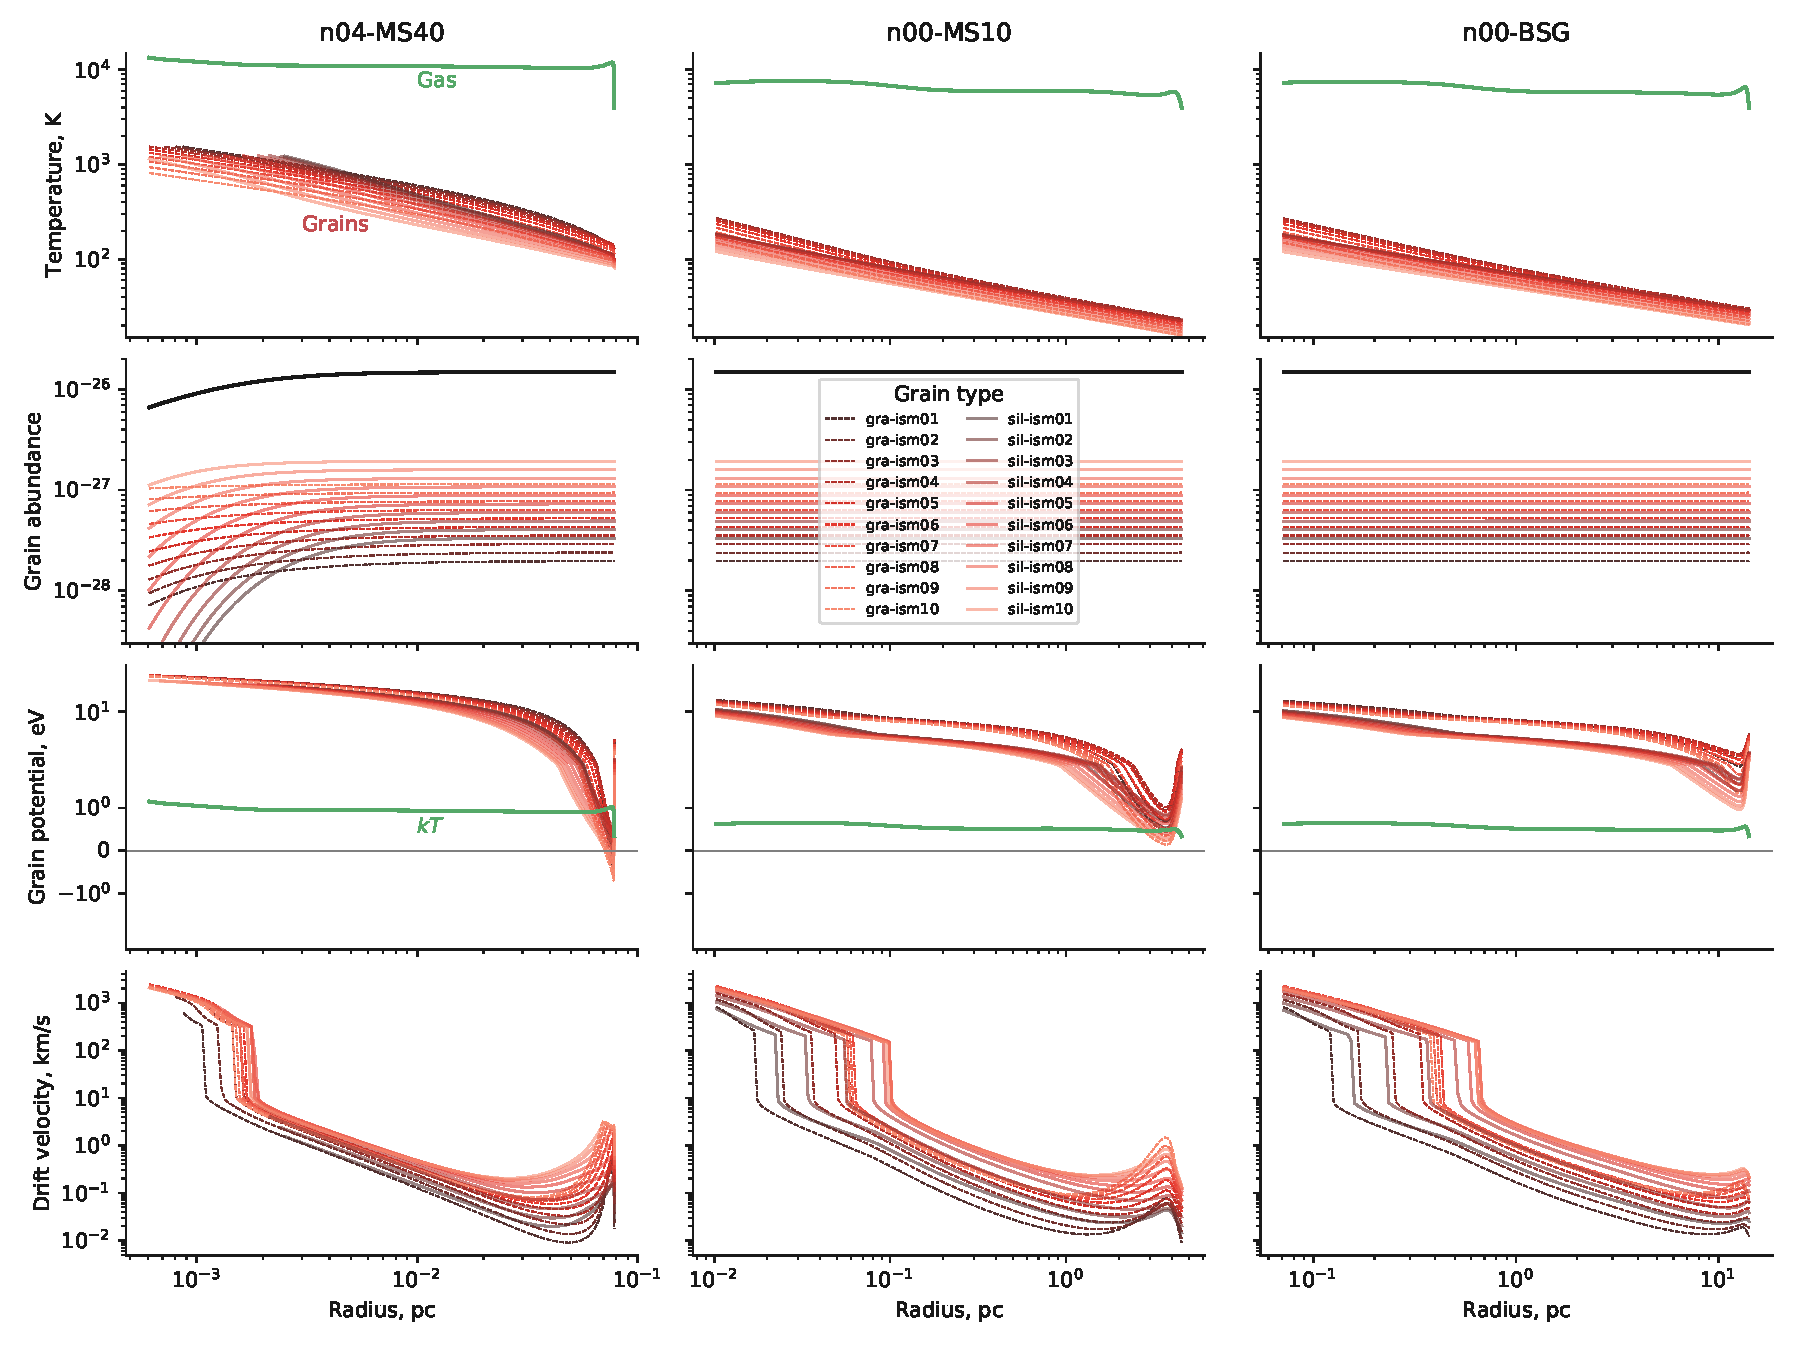
\includegraphics[width=\linewidth]{figs/multi-dustprops}
  \caption{Dust properties as a function of radius from star for three
    selected Cloudy simulations. (a)~\SI{40}{M_\odot} main-sequence star in
    medium of density \SI{e4}{cm^{-3}}. (b)~\SI{10}{M_\odot} main-sequence
    star in medium of density \SI{1}{cm^{-3}}. (c)~Blue supergiant
    star in medium of density \SI{1}{cm^{-3}}}.
  \label{fig:multi-dustprops}
\end{figure*}
Figure~\ref{fig:multi-dustprops} shows resultant radial profiles of
dust properties for representative simulations: grain temperature, grain
abundance, grain potential, and grain drift velocity.  Line types
correspond to the different size bins of graphite and silicate grains,
as indicated in the key from smallest to largest. The left hand panels
show results for a high-density (\(n = \SI{e4}{cm^{-3}}\)), compact
(\(R \approx \SI{0.1}{pc}\)) region around an early O~star, where the grain
temperature is very high, especially for the smaller silicate grains,
and sublimation significantly reduces the grain abundance in the inner
regions.  The remaining columns show low-density
(\(n = \SI{1}{cm^{-3}}\)), extended (\(R \sim \SI{10}{pc}\)) regions
around main-sequence and supergiant B-type stars, in which the grain
temperatures are much lower, ranging from \SIrange{20}{50}{K} in the
outer parts up to \SIrange{100}{200}{K} in the inner parts.

 
\begin{figure*}
  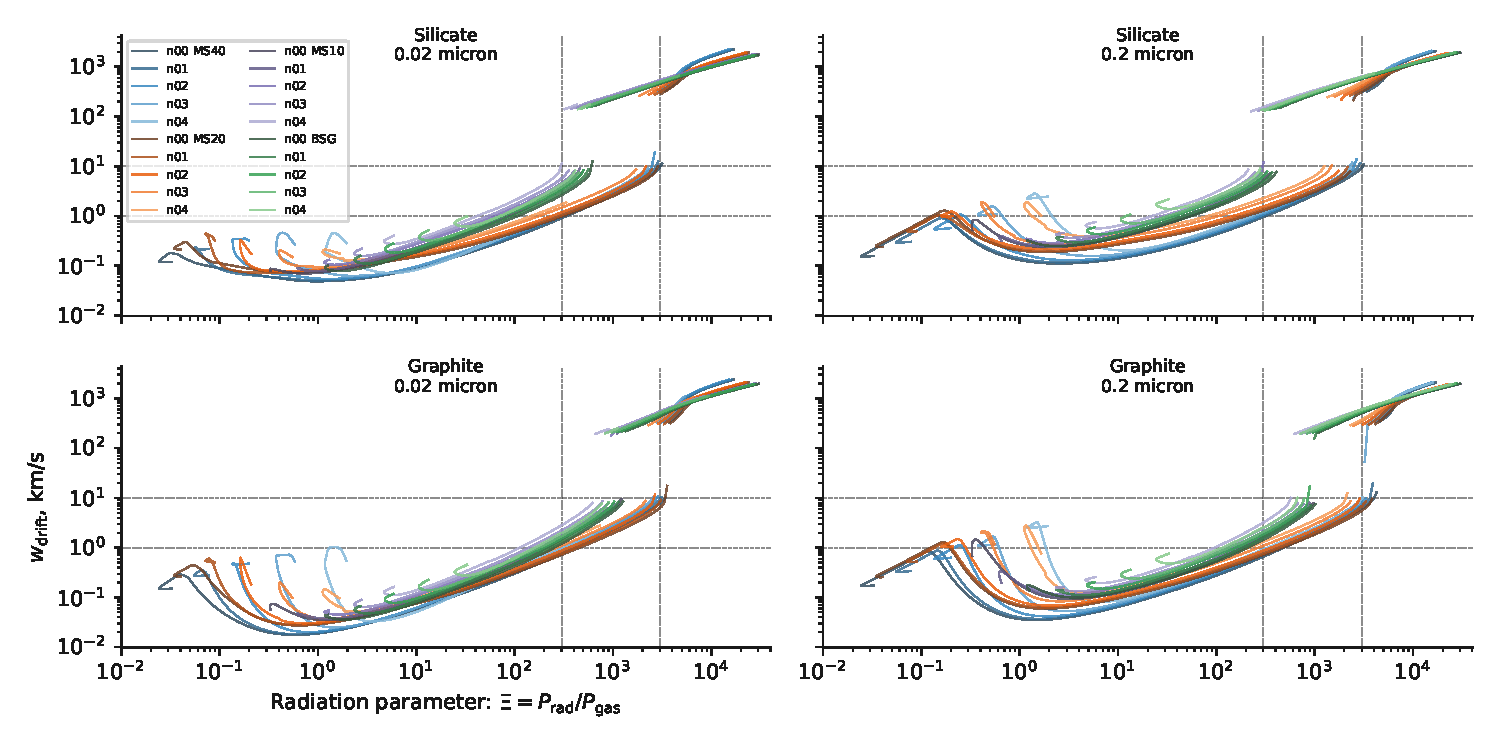
\includegraphics[width=\linewidth]{figs/drift-pratio-4panel}
  \caption{Drift velocity \(w\drift\) versus radiation parameter
    \(\Xi\). Each line represents a simulation with ambient density and
    stellar type as indicated in the key.  Results are shown for
    graphite and silicate grains of two different sizes.  The rip
    point, which corresponds to gas--grain decoupling, is the
    discontinuity in the curves at
    \(w\drift \approx \SI{10}{km.s^{-1}}\), indicated by the upper
    horizontal dashed line.  The vertical dashed lines show the narrow
    range of radiation parameter, \(\Xi = 1000 \pm \SI{0.5}{dex}\), that
    encompasses the rip point for all simulations. }
  \label{fig:drift-gn}
\end{figure*}

Unlike the strong differences in thermal properties, the radial
dependence of grain electrostatic potential (third row in
Fig.~\ref{fig:multi-dustprops}) is qualitatively similar for all the
simulations.  The grains are predominantly positively charged, with high
potentials (\(> 10\) times the thermal energy of gas particles) close
to the star due to the strong EUV and FUV photo-ejection.  The
potential falls to much lower values in the outer ionized region, as
the EUV flux falls off, and then climbs again at the ionization front
due to the fall in electron density, while the FUV photo-ejection
persists well into the neutral region.  There are small differences
between the simulations due to the increasing relative importance of the
EUV radiation for hotter stars, which leads to a deeper dip in the
potential just inside the ionization front for the \SI{40}{M_\odot} case,
even reaching negative values for some grain species.

Equilibrium drift velocity for each grain species is calculated in the
Cloudy simulations using the same theory \citep{Draine:1979a} as
outlined in \S~\ref{sec:drag-force-grains}.  The way that this is
implemented by default in Cloudy means that if the only solution at
the inner radius is a superthermal one, then the superthermal solution
branch (upper right corner of
Fig.~\ref{fig:gas-grain-drag-photoionized}) is followed as far as
possible through the outer spatial zones.  We have modified the code
so as to instead always prefer the slower subthermal branch whenever
multiple solutions are available.  This makes the most sense in our
context, where the grains are moving towards the star and so the
radiative force is gradually increasing from an initial low value.
Example results are shown in the bottom row of
Figure~\ref{fig:multi-dustprops} and again they are qualitatively
similar for all the simulations.  Close to the star, the radiation
force is higher than the upper limit on the Coulomb drag force
(eq.~[\ref{eq:fdrag-maximum}]), so that the equilibrium drift velocity
is exceedingly high.\footnote{Note that such high drift velocities are
  much higher than any realistic true relative velocity between grains
  and gas, since they are based on the assumption that the radiation
  force remains constant while the grain is accelerated, which is not
  the case near the rip point.  Instead, they are simply an indication
  that the gas and grains have completely decoupled.}.  As the radial
distance from the star increases, the radiation field is increasingly
diluted but the grain potential falls only slowly, so eventually one
reaches a point where an equilibrium between Coulomb drag and
radiation force can be established, which corresponds to a
discontinuity in the drift velocity.  This is the \textit{rip point}
discussed in \S~\ref{sec:gas-grain-separ}.  The drift velocity carries
on falling towards the outside of the \hii{} region, but then
increases again just inside the ionization front due to the drop in
grain potential there.

Both the charge balance and the force balance are essentially due to
competition between the photons and the charged particles that
interact with the grain.  It is therefore reasonable to surmise that
the gas--grain decoupling that occurs at the rip point might be
determined principally by the ratio of photons to gas particles.  We
test this hypothesis in Figure~\ref{fig:drift-gn}, where we
characterize the photon-gas ratio by a dimensionless radiation
parameter, \(\Xi\), equal to the radiation pressure divided by the gas
pressure.  Results are shown for four different grain types and for
all combinations of stellar parameters and ambient densities for which
we have run simulations.  It can be seen that the rip point does indeed
always occur at a similar value of \(\Xi \sim 1000\) for all simulations, albeit
with some variation according to the spectral type of the star and the
grain composition, as given in Table~\ref{tab:Xi-rip}.  The gas
density and grain size have very little influence on this critical
value \(\Xi_\dag\), with the only exception being the very smallest grains
(\(a < \SI{0.006}{\um}\), not illustrated), which show
\(\Xi_\dag \approx \num{e4}\), but such grains are only minor contributors to the
UV opacity (\(< 10\%\) in EUV and \(< 1\%\) in FUV, see
Fig.~\ref{fig:cloudy-ism-dust-opacity}).

\begin{figure}
  \centering
  \includegraphics[width=\linewidth]{figs/phi-versus-xi-annotate}
  \caption{Grain potential in thermal units (linear scale) versus
    radiation parameter (logarithmic scale). All densities and stellar
    types are shown, with line colors as in Fig.~\ref{fig:drift-gn}.
    Solid lines show silicate grains and dashed lines show graphite
    grains.  Line width increases with grain size (to reduce clutter,
    only every second size bin is shown).  The solid and dashed lines
    show the logarithmic fits discussed in the text.}
  \label{fig:phi-vs-Xi}
\end{figure}
Finally, Figure~\ref{fig:phi-vs-Xi} shows the slow dependence of grain
potential on radiation parameter for all the simulations on a linear
versus logarithmic scale.  The logarithmic fit of
equation~\eqref{eq:phi-vs-Xi}, most appropriate for carbon grains
around cooler stars, is shown by the solid line.  The dashed lines
show the modifications for silicate grains and for hotter stars (see
\S~\ref{sec:gas-grain-separ}).  Further details of the Cloudy dust
models are discussed in Appendix~\ref{sec:grain-temp-emiss}.



% Inner shock \dots no dust \dots proton Larmor radius very small, so
% no penetration across contact discontinuity

%%% Local Variables:
%%% mode: latex
%%% TeX-master: "dusty-bow-wave"
%%% End:
